
%\newtheorem{definition}[subsection]{Definition}
%\newtheorem{example}[subsection]{Example}
\newtheorem{cor}[subsection]{Corollary}
\newtheorem{pro}[subsection]{Proposition}
\newtheorem{theo}[subsection]{Theorem}
\newtheorem{lem}[subsection]{Lemma}
%\newtheorem{rem}[subsection]{Remark}

\definecolor{main}{HTML}{5989cf}    % setting main color to be used
\definecolor{sub}{HTML}{cde4ff}     % setting sub color to be used

\tcbset{
    sharp corners,
    colback = white,
    before skip = 0.2cm,    % add extra space before the box
    after skip = 0.5cm      % add extra space after the box
}                           % setting global options for tcolorbox

% You can copy any following box you like to your code.
\newtcolorbox{boxA}{
    fontupper = \bf,
    boxrule = 1.5pt,
    colframe = black % frame color
}

\newtcolorbox{boxB}{
    fontupper = \bf\color{main}, % font color
    boxrule = 1.5pt,
    colframe = main,
    rounded corners,
    arc = 5pt   % corners roundness
}
\newtcolorbox{boxC}{
    colback = sub, % background color
    boxrule = 0pt  % no borders
}

\newtcolorbox{boxD}{
    colback = sub, 
    colframe = main, 
    boxrule = 0pt, 
    toprule = 3pt, % top rule weight
    bottomrule = 3pt % bottom rule weight
}

\hypersetup{
    colorlinks=true,
    linkcolor=blue,
    filecolor=magenta,      
    urlcolor=cyan,
    pdftitle={Overleaf Example},
    pdfpagemode=FullScreen,
    }

\urlstyle{same}


\coursetitle{\mtthreeiii}{MT303}
\developers{Wyclife Rao}
\reviewers{Dr Irene Sitawa}
\modulenumber{9}
\modulename{Numerical Differentiation and Numerical Integration in Python}

% courses
\thispagestyle{empty}
\begin{tikzpicture}[overlay,remember picture,font=\sffamily\bfseries]
 \draw[ultra thick,c4,name path=big arc] ([xshift=-2mm]current page.north) arc(150:285:11) coordinate[pos=0.225] (x0);
 \begin{scope}
  \clip ([xshift=-2mm]current page.north) arc(150:285:11) --(current page.north east);
  \fill[c4!50,opacity=0.25] ([xshift=4.55cm]x0) circle (4.55);
  \fill[c4!50,opacity=0.25] ([xshift=3.4cm]x0) circle (3.4);
  \fill[c4!50,opacity=0.25] ([xshift=2.25cm]x0) circle (2.25);
  \draw[ultra thick,c4!50] (x0) arc(-90:30:6.5);
  \draw[ultra thick,c4] (x0) arc(90:-30:8.75);
  \draw[ultra thick,c4!50,name path=arc1] (x0) arc(90:-90:4.675);
  \draw[ultra thick,c4!50] (x0) arc(90:-90:2.875);
  \path[name intersections={of=big arc and arc1,by=x1}];
  \draw[ultra thick,c4,name path=arc2] (x1) arc(135:-20:4.75);
  \draw[ultra thick,c4!50] (x1) arc(135:-20:8.75);
  \path[name intersections={of=big arc and arc2,by={aux,x2}}];
  \draw[ultra thick,c4!50] (x2) arc(180:50:2.25);
 \end{scope} 
 \path[decoration={text along path,text color=c4,
                 raise = -2.8ex,
                 text  along path,
                 text = {},%|\sffamily\bfseries|02/18/2019
                 text align = center,
             },
             decorate
         ] ([xshift=-2mm]current page.north) arc(150:245:11);
 %
 \newcommand\add{4cm}
 \begin{scope}%[shift={(5,0)}]
  \path[clip,postaction={fill=c3}]
  ([xshift=2cm+\add,yshift=-8cm]current page.center) rectangle ++ (4.6,7.7);
  \draw[c5,ultra thick,fill=c2] ([xshift=0.5cm+\add,yshift=-8cm]current page.center)
   ([xshift=0.5cm+\add,yshift=-8cm]current page.center)  arc(180:60:2)
    |- ++ (-3,6) --cycle;
  \draw[ultra thick,c5] ([xshift=-1.5cm+\add,yshift=-8cm]current page.center) 
  arc(180:0:2);
  \draw[ultra thick,c5] ([xshift=0.5cm+\add,yshift=-8cm]current page.center) 
  arc(180:0:2);
  \draw[ultra thick,c5] ([xshift=2.5cm+\add,yshift=-8cm]current page.center) 
  arc(180:0:2);
  \draw[ultra thick,c5] ([xshift=4.5cm+\add,yshift=-8cm]current page.center) 
  arc(180:0:2);
  \fill[white] ([xshift=2.5cm+\add,yshift=-8cm]current page.center) +(60:2) circle(1.5mm)
  node[above
  right=0mm,text=c5!80!black]{$\rho:=\dfrac{1+\sqrt{-3}}{2}$};
 \end{scope}
 %
 \fill[c1] ([xshift=2cm+\add,yshift=-8cm]current page.center) rectangle ++ (-30.7,7.7);
 \node[text=white,anchor=west,scale=2.3,inner sep=0pt] at
 ([xshift=-10cm,yshift=-1.8cm]current page.center) {\color{ulabgold} LEARNING};
 \node[text=white,anchor=west,scale=5,inner sep=0pt] at
 ([xshift=-10cm,yshift=-3.25cm]current page.center) {MODULE \dpmdnumber};
 \node[text=white,anchor=west,scale=2.5,inner sep=0pt,text width=.4\textwidth] at
 ([xshift=-10cm,yshift=-6cm]current page.center) {\dpmdname};
 \node[text=white,anchor=east,scale=2,inner sep=0pt] at
 ([xshift=5.7cm,yshift=-7.5cm]current page.center) {\color{ulabgold}The Open University of Kenya};
 %
% \draw[gray,line width=5mm] 
% ([xshift=2mm,yshift=-1mm]current page.south west) rectangle ([xshift=-2mm,yshift=1mm]current
% page.north east);
\end{tikzpicture}

%\newpage
\pagenumbering{roman}
\thispagestyle{empty}%firstpage


\begin{center}
\vspace*{2cm}
{\Huge\bf BACHELOR OF TECHNOLOGY EDUCATION}\\[3cm]  


%{\fontsize{80}{40}\selectfont \dpcoursecode}\\[2cm]
%
%{\fontsize{30}{40} \selectfont \dpcoursename}\\[2cm]

%\rule{\textwidth}{1pt}
%\vspace{2cm}

%{\fontsize{40}{40}\selectfont \bf Module~\dpmdnumber}\\[2cm]
%
%{\fontsize{30}{40}\selectfont \bf \dpmdname}\\

\vfill
\begin{flushright}
\begin{minipage}{.6\textwidth}
\begin{tcolorbox}%[text ]
\begin{tabular}{ll}%\hline
\subtitle{Developed by:}&\displaydevelopers\\
&\\
\subtitle{Reviewed by:}&\makecell[l]{\displayreviewers}\\
\end{tabular}
\end{tcolorbox}
\end{minipage}\hspace*{-3.5cm}
\end{flushright}
\vspace*{-2.5cm}
\end{center}

\newpage
\thispagestyle{empty}
\null
\vfill
{\renewcommand\arraystretch{1.5}
\begin{tabular}{|l|l|}\hline
\subtitle{Programme Title} & Bachelor of Technology Education \\\hline
\subtitle{Course Title} & \fullcoursename\\\hline
\subtitle{Learning Module number} & Module \dpmdnumber\\\hline
\subtitle{Learning module title} & \dpmdname \\\hline
\subtitle{Module Developer} & \displaydevelopers\\\hline
\subtitle{Reviewed by} & \displayreviewers\\\hline
%\subtitle{Vision} & \vision\\\hline
%\subtitle{Audience description} & \\\hline
\end{tabular}}
\clearpage

%\section{COURSE LEARNING GUIDE}


\subsection*{Preparing for Online and Distance Learning}

This course offers you the opportunity to enter an online space where you can engage with fellow students at the university. The online forums, exercises, tasks and materials have been designed by the course facilitators in such a way that you can draw directly from their knowledge and share in their scholarly interest in online learning and assessment

We hope you will use your access to this virtual classroom to raise all your questions on the course module, to build a network great learners and to share your own thoughts and experiences to the benefit of your fellow students.

   
There are a number of steps you can take to ensure you are well prepared to make the most of this learning opportunity. This resource should prompt you to consider the following:


 \begin{enumerate}[label=\cb$\square$]
   \item How can you best prepare the space where you expect you will spend most of your time engaging in online learning (i.e. in your home or office, or even during your commute to work or whilst traveling)?
  \item   What can you do to ensure you keep working through the course material, even when you do not have Internet access?
    \item How can you familiarise yourself with the course layout, in order to be able to navigate through the steps with ease?
    \item What are the communication strategies and best practices you could consider to best engage with your fellow students and the course facilitators?
    \item What do you do when you need academic or technical support?

 \end{enumerate} 

\subsection*{General Module Guide}

The authors of this module believe that imparting knowledge should always be a mutual relationship between the students and the teachers. Students can actively construct knowledge through experiences gained in reading and answering the learning modules.

You should take time to read everything written in the module, actively and religiously solve all the exercises included to finish this course and be able to gain all the competencies and skills expected to demonstrate the learning outcomes as stated in this course. If you finish with full confidence that you understand and can apply all the knowledge you gain in this course, then you are sure to succeed in tackling the next higher subjects in your chosen course.

In this course, you will be taught not only the knowledge you need to demonstrate your learning outcomes, but you will also gain discipline, perseverance, higher thinking skills, and resourcefulness that would help strengthen your foundation to succeed in life. To successfully finish the course, you must follow the guides set forth in using this module.


\begin{description}[{format=\textcolor{ulabblue}}]
\item[STUDY ENVIRONMENT.]\leavevmode\\
Before engaging into the module, make sure that you are comfortable enough and diminish distractions. Make sure that you develop a study routine to perform and accomplish all the activities set forth by the module.
%\newpage

\item[MODE OF DELIVERY.]\leavevmode\\
Students are required to get a access a digitised copy of the module from the Virtue Learning Environment. As an open and distance learner, you should be able to learn independently and optimise the learning modes and environment available to you as much of  the delivery of all the lessons will be done asynchronously. Your success will greatly depend on your self-motivation and discipline to get your work done without your instructor to remind you from time to time.

\item[STUDY SCHEDULE.] \leavevmode\\
Remember that you have other subjects to attend to, hence, you must manage your time so that you will not be left behind in any of them. Create your own learning plan for each course to make sure that you can perform all the activities. Do not procrastinate your work, remember that time wasted can never be retrieved back. Make sure that even if you are at home, you are a student enrolled in a program, where the learning of all its courses greatly depends on your will to learn as the materials you need are all in your hands. So always be aware of your daily tasks.

\item[PRACTICE EXERCISE.]\leavevmode\\
To measure your learning from your reading, you are given practice exercises which you are supposed to answer daily. This will prepare you in performing your main task.

\item[ONLINE GROUP CHAT.]\leavevmode\\
I am going to create an online Discussion Forum and QA Forum  on the VLE.  This will serve as a room for discussion on the topics and activities found in your module.

\item[RECOMMENDED REFERENCES FOR SUPPLEMENTARY READING.]\leavevmode\\
You are given links that you need to access online. These links are online references such as e-books, online activities, and tutorial videos of the topic. These are other references you can use to further understand the topic and gain additional knowledge and skills.

\item[MAIN TASK.]\leavevmode\\
You are given a task that will require you to apply the knowledge and skills you learned from the module. This can be a group or individual activity which will measure your higher order thinking skills you acquired throughout the topic.

\item[RUBRICS. ]\leavevmode\\
This is a tool to guide you in performing your main task. Through this, you will be able to know the specific indicators that should be found in your task. This is to assess your constructive behaviour towards your learning application. You will be rated according to a 4-point scale shown below.
\begin{center}
{\color{ulabgold} \bf 4 − Excellent\quad\quad   3 −Good\quad\quad    2 − Fair \quad\quad  1 −Poor}
\end{center}
\item[REFLECTIONS.]\leavevmode\\
Writing your reflection will be a passageway to express your experiential learning in using this module. In your honest recall, write everything that you think happened to you during your learning experience in this module. Use the guide questions below:
\begin{description}[{format=\textcolor{ulabblue}}]
\item[First paragraph. ]\leavevmode\\
How was your learning experience? Maybe you can consider describing the effect of the parts of the module (sequence, discussions, examples, practice exercises, online activities, and the main task) in your learning experience. You can point out the strength and weakness of each part so that we can consider it for future improvement of this instructional material.
\item[Second paragraph.  ]\leavevmode\\
What did you learn? Did you successfully acquire the learning outcomes?

\item[Third paragraph.]\leavevmode\\
How can you use what you learned in the future?
\end{description}
\end{description}

\section{ASSESSMENT  TASKS \& EXAMINATION   RULES AND GUIDELINES}

\begin{enumerate}[label=\cb\arabic*.]
\item {\cb SUBMISSION OF ASSESSMENT TASTS.}

Since mathematical skills are best acquired through constant practice, you are encouraged to answer at least two (2) exercises a day. These practice exercises will not be graded but it will help you develop your thinking skills which will prepare you in the performance of your main tasks. You are required to submit your practice exercises every week.
\begin{center} {\cg Usually submission deadlines are set on Saturday 11:59PM EAT} \end{center}

\item  {\cb GROUP CHAT.}

You can post questions, solutions, and comment to other's post. Please be reminded that our group chat is exclusive only for discussion on topics related to this course. Everyone is required to actively participate in the discussions. Also, trolling is highly discouraged. Always observe proper online etiquettes when participating in discussions.
\begin{center} {\cb RULE OF THUMB: ALWAYS THINK BEFORE YOU CLICK} \end{center}

\item  {\cb MAIN TASK. }

Complete documentation during the preparation of your task is required to ensure that every member of the group participated and contributed in the task. May it be photos or screenshots of your virtual meetings or group works. You are going to submit it as attachment of your main task the same way as the practice exercises.



\item {\cb RECOMMENDED REFERENCES FOR SUPPLEMENTARY READING.} 

You can explore online for other references that is related to the topic to gain additional information about the topic. Do not share or post inappropriate materials online or even privately.
\end{enumerate}

\subsection*{Requirements to pass the course}

Compiled Continuous  Assignment/Activities and Tasks  with Final Performance Examination.

\subtitle{Grading System}
\begin{center}
{\renewcommand\arraystretch{1.5}
\begin{tabular}{|l|c|}\hline
Continuous Activities and Tasks  &  50\%\\\hline
Final Performance Examination. &  50\%\\\hline
\end{tabular}
}
\end{center}
%\newpage










%\subsection{INTRODUCTORY MESSAGE}

%A warm welcome to \;  \fullcoursename, {\bf Module on \dpmdname}.



%By this module learning resource, we aim to enable you  achieve the relevant competencies, depict skill, action and purpose successfully. 
 

%It has been designed to provide you with fun and meaningful opportunities for guided and independent learning at your own pace and time. You will be enabled to process the contents of the learning material while being an active learner. Your academic success lies in your own hands.  This module has the following parts and corresponding icons:





{
\renewcommand\arraystretch{4}
\begin{longtblr}{
width=\linewidth,
 colspec={ Q[1,c,f] Q[1.5,r,m] Q[4,l,m] },
%row{1} = { font=\bfseries },
% rowhead = 1,
  caption={ }, 
  label={ },
  rowsep = 4pt,
  hlines = {ulabblue!20, 1pt},
  vlines = {ulabblue!20, 1pt},
}

\includegraphics[width=2cm]{img/audience} & {\bf AUDIENCE}  &  This is a description of a target audience.   \\
{\fontsize{40}{30}\selectfont\color{ulabblue}\faCogs}& {\bf MODULE DESCRIPTION} & 
This part explains the importance of the topics discussed in the module. It will also give you a sneak peek of what you will learn and what is expected from you at the end of the module.\\

\includegraphics[width=2cm]{img/target.png} &  {\bf  EXPECTATION} & These are what you will be able to know after completing the lessons in the module\\

\includegraphics[width=2cm]{img/preactivities} & {\bf PRE-ACTIVITY} &
This activity is to get you set, activate and engage schema to learn the module. Through this activity, you will know the relevance of this activity to the topic that will be discussed in the module.\\

\includegraphics[width=2cm]{img/pretest} &  {\bf PRE - ASSESSMENT} & This will measure your prior knowledge and the concepts to be mastered throughout the lesson. \\

\includegraphics[width=1.7cm]{img/rewind} &  {\bf  RECAP} & This section will measure what learnings and skills that you understand from the previous lesson.\\

\includegraphics[width=1.5cm]{img/lesson} &  {\bf  LESSON} & This section will discuss the topic for this module.\\

\includegraphics[width=2cm]{img/activities} &  {\bf  ACTIVITIES} & This is a set of activities you will perform.\\

\includegraphics[width=2cm]{img/summary} &  {\bf  WRAP UP} & This section summarizes the concepts and applications of the lessons.\\

\includegraphics[width=2cm]{img/discussion}& {\bf DISCUSSIONS} &
This is the meat of the module. The discussion is aligned to the topic learning outcomes that is expected of you to acquire at the end of the module.\\

\includegraphics[width=1.8cm]{img/value} &  {\bf  VALUING} & This part will check the integration of values in the learning competency you will take home.\\

\includegraphics[width=1.8cm]{img/posttest} &  {\bf  POST - ASSESSMENT} & This will measure how much you have learned from the entire module.\\

\includegraphics[width=1.8cm]{img/selfreflect} & {\bf REFLECTION }
&
This part is for you to share your thoughts by writing your reflection, make sure to check your grammar and spelling to ensure the readability and so that it will not alter the thought being delivered. 
\end{longtblr}
}









%\vfill

\audience
\begin{oldactivity}{Audience Description}{
\includegraphics[width=22mm]{img/audience}}{}
This module is offered to all students taking the Bachelor of Technology Education. As an open and distance learner, you should be able to learn independently and optimise the learning modes and environment available to you. Before you begin this course, please confirm the course material, the course requirements and how the course is conducted.
\end{oldactivity}
%\newpage
\pagenumbering{arabic}



\mddescription
This module guides you into a detailed discussion of the concepts of numerical differentiation and numerical integration using python. Specifically you will learn about
\begin{itemize}
\item finite difference approximation of derivatives and approximation of higher order derivatives
\item numerical differentiation with noise
\item Riemann's integral, trapezoidal rule and Simpson's rule
\item Computing integrals in python. 
\end{itemize}
%\expectations
%\begin{objenumerate}
%
%\end{objenumerate}

\begin{mlos}
\item Identify composite trapezoidal and midpoint methods for numerical integration.
\item Explain the concept of vectorization and its role in computational speed.
\item Perform double and triple integrals using numerical methods and vectorized code.
\item Measure and compare computational speed for different numerical integration implementations. 
\end{mlos}

\section{Finite Difference and Higher Order Derivatives in Python}
\videolesson
\begin{selfvideo}[1]
%LESSON 3: 
This video presents a discussion on finite differences approximation of derivatives and approximation of higher order derivatives in python. Follow the discussion and then solve the problems in the subsequent quiz.
\end{selfvideo}
%\begin{boxB}Question: \end{boxB}
%A {\bf numerical grid} is an evenly spaced set of points over the domain of a function, over some interval. The {\bf spacing} or {\bf step size} of a numerical grid is the distance between adjacent points on the grid. For the purpose of this text, if $x$ is a numerical grid, then $x_j$ is the $j$th point in the numerical grid and $h$ is the spacing between $x_{j-1}$ and $x_j$
%
%The following figure shows an example of a numerical grid.
%\begin{figure}[h]
%\centering
%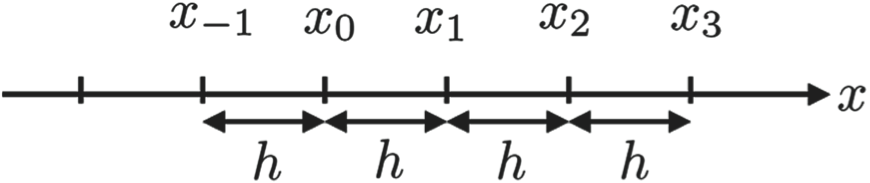
\includegraphics[width=10cm]{20.01.01-Numerical_grid}
%\caption{}
%\label{20.01.01-Numerical_gridfig1}
%\end{figure}
%
%\subsection*{Finite Difference Approximating Derivatives}
%The derivative $f′(x)$ of a function $f(x)$ at the point $x=a$ is defined as:
%\[f′(a)=\lim_{x\rightarrow a}\frac{f(x)-f(a)}{x-a}\]
%The derivative at $x=a$ is the slope at this point. In {\bf finite difference} approximations of this slope, we can use values of the function in the neighborhood of the point $x=a$ to achieve the goal. There are various finite difference formulas used in different applications, and three of these, where the derivative is calculated using the values of two points, are presented below.
%
%The {\bf forward difference} is to estimate the slope of the function at $x_j$ using the line that connects $(x_j,f(x_j))$ and $(x_{j+1},f(x_{j+1}))$:
%\[f′(x_j)=\frac{f(x_{j+1})-f(x_j)}{x_{j+1}-x_j}\]
%The {\bf backward difference} is to estimate the slope of the function at $x_j$ using the line that connects $(x_{j-1},f(x_{j-1}))$ and $(x_j,f(x_j))$:
%\[f′(x_j)=\frac{f(x_{j})-f(x_{j-1})}{x_{j}-x_{j-1}}\]
%The {\bf central difference} is to estimate the slope of the function at $x_j$ using the line that connects $(x_{j-1},f(x_{j-1}))$ and $(x_{j+1},f(x_{j+1}))$:
%\[f′(x_j)=\frac{f(x_{j+1})-f(x_{j-1})}{x_{j+1}-x_{j-1}}\]
%The following figure illustrates the three different type of formulas to estimate the slope.
%\begin{figure}[h]
%\centering
%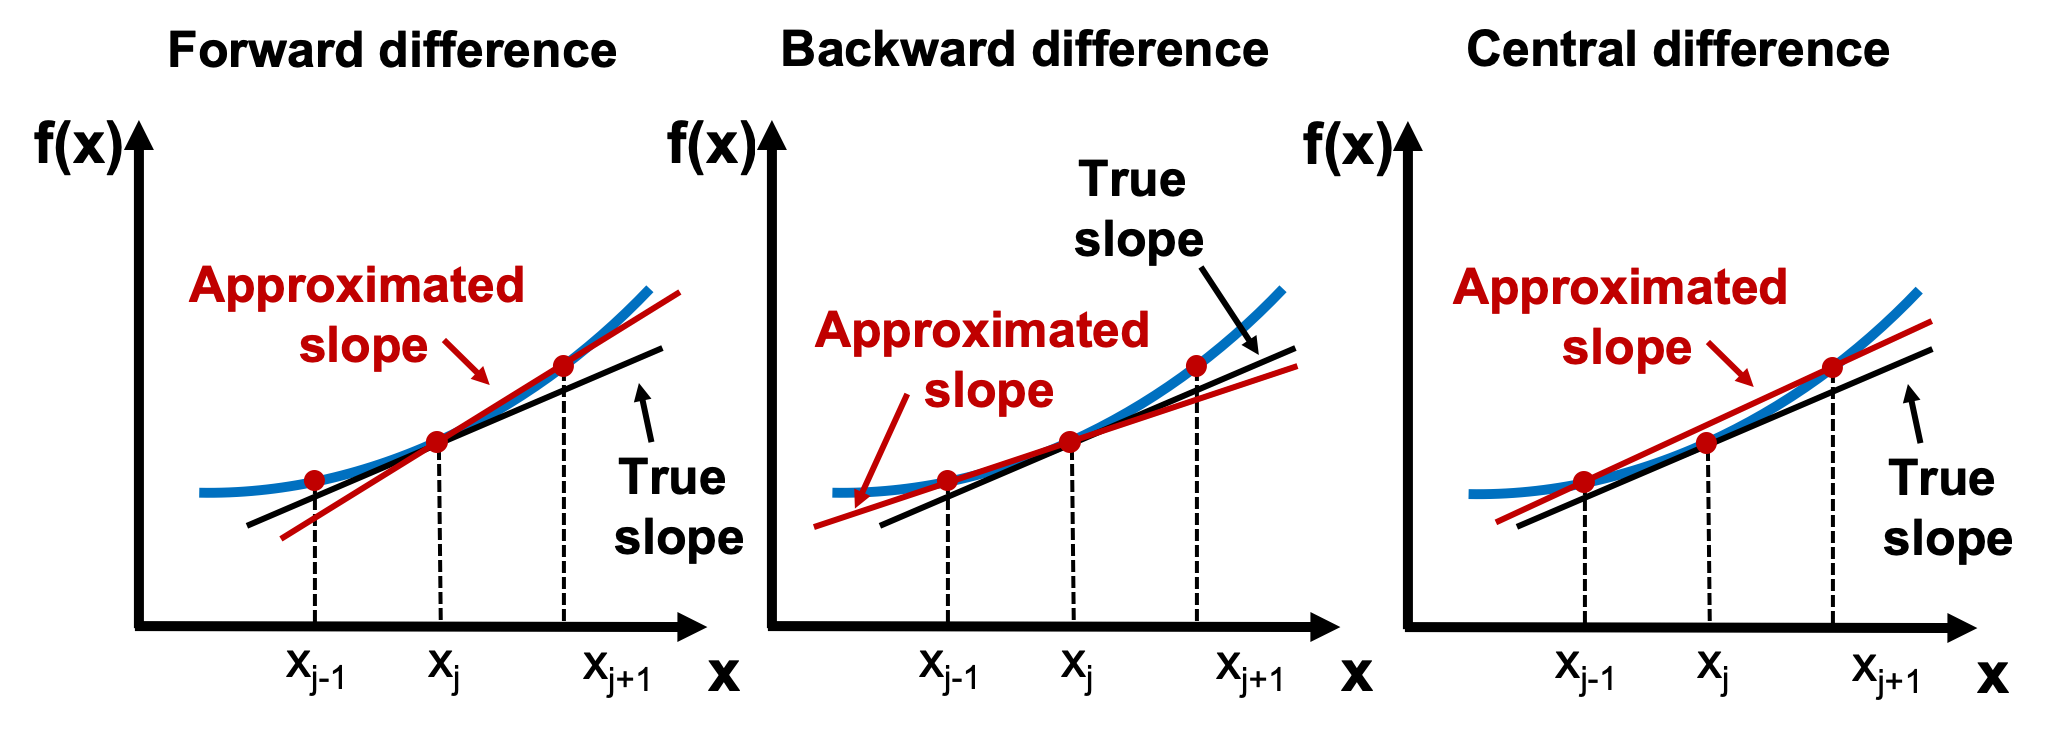
\includegraphics[width=14cm]{20.02.01-Finite-difference}
%\caption{}
%\label{20.02.01-Finite-differencefig2}
%\end{figure}
%
%\subsubsection*{Finite Difference Approximating Derivatives with Taylor Series}
%To derive an approximation for the derivative of $f$, we return to Taylor series. For an arbitrary function $f(x)$ the Taylor series of $f$ around $a=x_j$ is 
%\[f(x)=\frac{f(x_j)(x-x_j)^0}{0!}+\frac{f'(x_j)(x-x_j)^1}{1!}+\frac{f''(x_j)(x-x_j)^2}{2!}+\frac{f''(x_j)(x-x_j)^3}{3!}+\cdots\]
%If $x$ is on a grid of points with spacing $h$, we can compute the Taylor series at $x=x_{j+1}$ to get
%\[f(x_{j+1})=\frac{f(x_j)(x_{j+1}-x_j)^0}{0!}+\frac{f'(x_j)(x_{j+1}-x_j)^1}{1!}+\frac{f''(x_j)(x_{j+1}-x_j)^2}{2!}+\frac{f''(x_j)(x_{j+1}-x_j)^3}{3!}+\cdots\]
%Substituting $h=x_{j+1}−x_j$ and solving for $f'(x_j)$ gives the equation
%\[f'(x_j)=\frac{f(x_{j+1})-f(x_j)}{h}+\left(-\frac{f''(x_j)h}{2!}-\frac{f'''(x_j)h^2}{3!}-\cdots\right).\]
%The terms that are in parentheses, $-\frac{f''(x_j)h}{2!}-\frac{f'''(x_j)h^2}{3!}-\cdots,$ , are called higher order terms of $h$. The higher order terms can be rewritten as
%\[-\frac{f''(x_j)h}{2!}-\frac{f'''(x_j)h^2}{3!}-\cdots=h(\alpha+\epsilon(h),\]
%where $\alpha$ is some constant, and $\epsilon(h)$ is a function of $h$ that goes to zero as $h$ goes to $0$. We use the abbreviation $O(h)$ for $h(\alpha+\epsilon(h))$, and in general, we use the abbreviation $O(h^p)$  to denote $h^p(\alpha+\epsilon(h))$.
%
%Substituting $O(h)$ into the previous equations gives
%\[f'(x_j)=\frac{f(x_{j+1})-f(x_j)}{h}+O(h).\]
%This gives the {\bf forward difference} formula for approximating derivatives as
%\[f'(x_j)\approx\frac{f(x_{j+1})-f(x_j)}{h},\]
%and we say this formula is $O(h)$.
%
%Here, $O(h)$ describes the {\bf accuracy} of the forward difference formula for approximating derivatives. For an approximation that is $O(h^p)$, we say that $p$ is the order of the accuracy of the approximation. With few exceptions, higher order accuracy is better than lower order. To illustrate this point, assume $q<p$. Then as the spacing, $h>0$, goes to $0$, $h^p$ goes to $0$ faster than $h^q$. Therefore as $h$ goes to $0$, an approximation of a value that is $O(h^p)$ gets closer to the true value faster than one that is $O(h^q)$.
%
%By computing the Taylor series around $a=x_j$ at $x=x_{j-1}$ and again solving for $f'(x_j)$, we get the {\bf backward difference} formula
%\[f'(x_j)\approx\frac{f(x_j)-f(x_{j-1})}{h},\]
%which is also $O(h)$.
%
%Intuitively, the forward and backward difference formulas for the derivative at $x_j$ are just the slopes between the point at $x_j$ and the points $x_{j+1}$ and $x_{j-1}$, respectively.
%
%We can construct an improved approximation of the derivative by clever manipulation of Taylor series terms taken at different points. To illustrate, we can compute the Taylor series around $a=x_j$ at both $x_{j+1}$ and $x_{j-1}$. Written out, these equations are
%\[f(x_{j+1})=f(x_j)+f'(x_j)h+\frac12f''(x_j)h^2+\frac16f'''(x_j)h^3+\cdots\]
%and
%\[f(x_{j-1})=f(x_j)-f'(x_j)h+\frac12f''(x_j)h^2-\frac16f'''(x_j)h^3+\cdots\]
%Subtracting the formulas above gives
%\[f(x_{j+1})-f(x{j-1})=2f'(x_j)+\frac23f'''(x_j)h^3+\cdots,\]
%which when solved for $f'(x_j)$ gives the central difference formula
%\[f'(x_j)\approx\frac{f(x_{j+1})-f(x_{j-1})}{2h}.\]
%Because of how we subtracted the two equations, the $h$ terms canceled out; therefore, the central difference formula is $O(h^2)$, even though it requires the same amount of computational effort as the forward and backward difference formulas! Thus the central difference formula gets an extra order of accuracy for free. In general, formulas that utilize symmetric points around $x_j$, for example $x_{j-1}$ and $x_{j+1}$, have better accuracy than asymmetric ones, such as the forward and background difference formulas.
%
%The following figure shows the forward difference (line joining$ (x_j,y_j)$ and $(x_{j+1},y_{j+1})$), backward difference (line joining $(x_j,y_j)$ and $(x_{j-1},y_{j-1})$), and central difference (line joining $(x_{j-1},y_{j-1})$ and $(x_{j+1},y_{j+1})$) approximation of the derivative of a function $f$. As can be seen, the difference in the value of the slope can be significantly different based on the size of the step $h$ and the nature of the function.
%\begin{figure}[h]
%\centering
%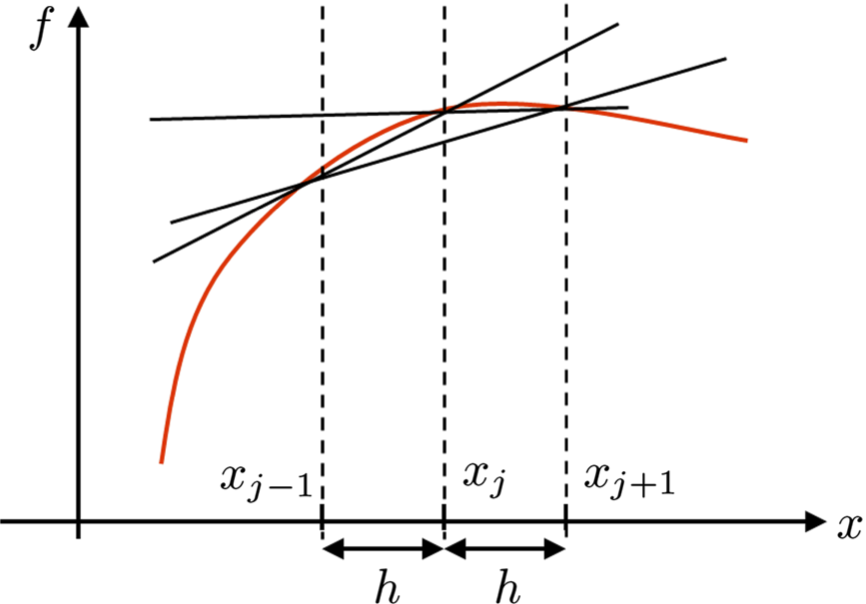
\includegraphics[width=10cm]{20.02.01-Forward_difference}
%\caption{}
%\label{20.02.01-Forward_differencefig3}
%\end{figure}
%
%\begin{example}
%Take the Taylor series of $f$ around $a=x_j$ and compute the series at $x=x_{j-2}$, $x_{j-1}$, $x_{j+1}$, $x_{j+2}$. Show that the resulting equations can be combined to form an approximation for $f'(x_j)$ that is $O(h^4)$.
%\end{example}
%
%\begin{mysolution}
%First, compute the Taylor series at the specified points.
%\[\begin{split}
%f(x_{j-2})&=f(x_j)-2hf'(x_j)+\frac{4h^2f''(x_j)}{2}-\frac{8h^3f'''(x_j)}{6}+\frac{16h^4f''''(x_j)}{24}-\frac{32h^5f'''''(x_j)}{120}+\cdots\\[2mm]
%f(x_{j-1})&=f(x_j)-hf'(x_j)+\frac{h^2f''(x_j)}{2}-\frac{h^3f'''(x_j)}{6}+\frac{h^4f''''(x_j)}{24}-\frac{h^5f'''''(x_j)}{120}+\cdots\\[2mm]
%f(x_{j+1})&=f(x_j)+hf'(x_j)+\frac{h^2f''(x_j)}{2}+\frac{h^3f'''(x_j)}{6}+\frac{h^4f''''(x_j)}{24}+\frac{32h^5f'''''(x_j)}{120}+\cdots\\[2mm]
%f(x_{j+2})&=f(x_j)+2hf'(x_j)+\frac{4h^2f''(x_j)}{2}+\frac{8h^3f'''(x_j)}{6}+\frac{16h^4f''''(x_j)}{24}+\frac{32h^5f'''''(x_j)}{120}+\cdots
%\end{split}\]
%To get the $h^2$, $h^3$, and $h^4$ terms to cancel out, we can compute
%\[f(x_{j-2})-8f(x_{j-1})+8f(x_{j-1})-f(x_{j+2})=12hf'(x_j)-\frac{48h^5f'''''(x_j)}{120}\]
%which can be rearranged to
%\[f'(x_j)=\frac{f(x_{j-2})-8f(x_{j-1})+8f(x_{j-1})-f(x_{j+2})}{12h}+O(h^4).\]
%This formula is a better approximation for the derivative at $x_j$ than the central difference formula, but requires twice as many calculations.
%\end{mysolution}


Python uses the following command to compute finite differences directly: for a vector $f$, the command $d=np.diff(f)$ produces an array $d$ in which the entries are the differences of the adjacent elements in the initial array $f$. In other words $d(i)=f(i+1)-f(i)$.



When using the command $np.diff$, the size of the output is one less than the size of the input since it needs two arguments to produce a difference.


\begin{example}
Consider the function f(x)=cos(x)
. We know the derivative of cos(x)
 is −sin(x)
. Although in practice we may not know the underlying function we are finding the derivative for, we use the simple example to illustrate the aforementioned numerical differentiation methods and their accuracy. The following code computes the derivatives numerically.
\end{example}

\begin{boxB}
import numpy as np\\
import matplotlib.pyplot as plt\\
plt.style.use('seaborn-poster')\\
%matplotlib inline\\
\end{boxB}

\begin{boxB}
\# step size\\
$h = 0.1$\\
\# define grid\\
$x = np$.arange(0, 2*np.pi, h) \\
\# compute function\\
$y = np.cos(x)$ \\
\\
\# compute vector of forward differences\\
forward\_diff = np.diff(y)/h \\
\# compute corresponding grid\\
$x_diff = x[:-1:]$ \\
\# compute exact solution\\
exact\_solution = -np.sin(x\_diff) \\
\\
\# Plot solution\\
plt.figure(figsize = (12, 8))\\
plt.plot(x\_diff, forward\_diff, '--', \textbackslash \\
         \hspace*{2cm}label = 'Finite difference approximation')\\
plt.plot(x\_diff, exact\_solution, \textbackslash \\
         \hspace*{2cm}label = 'Exact solution')\\
plt.legend()\\
plt.show()\\
\\
\# Compute max error between \\
\# numerical derivative and exact solution\\
max\_error = max(abs(exact\_solution - forward\_diff))\\
print(max\_error)\\
\end{boxB}
\newpage
\begin{figure}[h]
\centering
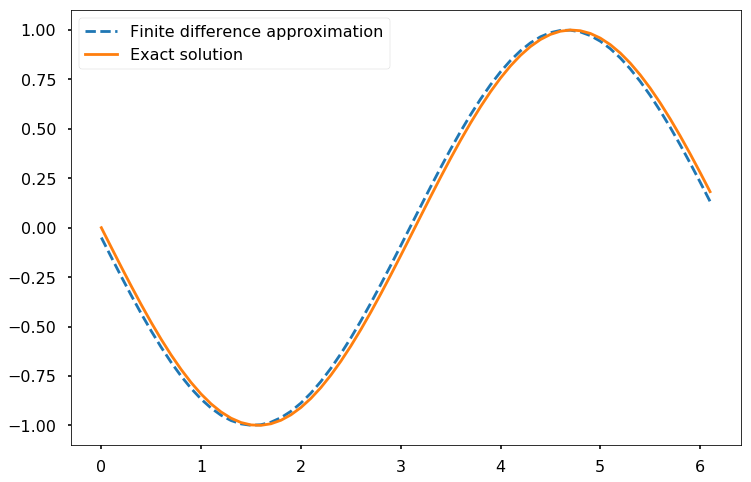
\includegraphics[width=12cm]{chapter20.02-Finite-Difference-Approximating-Derivatives_5_0}
\caption{}
\label{}
\end{figure}

0.049984407218554114

As the above figure shows, there is a small offset between the two curves, which results from the numerical error in the evaluation of the numerical derivatives. The maximal error between the two numerical results is of the order $0.05$ and expected to decrease with the size of the step.

As illustrated in the previous example, the finite difference scheme contains a numerical error due to the approximation of the derivative. This difference decreases with the size of the discretization step, which is illustrated in the following example.

\begin{example}
The following code computes the numerical derivative of $f(x)=\cos(x)$ using the forward difference formula for decreasing step sizes, $h$. It then plots the maximum error between the approximated derivative and the true derivative versus $h$ as shown in the generated figure.

\begin{boxB}
\# define step size\\
$h = 1$\\
\# define number of iterations to perform\\
iterations = 20 \\
\# list to store our step sizes\\
step\_size = [] \\
\# list to store max error for each step size\\
max\_error = [] \\
\\
for i in range(iterations):\\
    \hspace*{0.5cm}\# halve the step size\\
    \hspace*{0.5cm}h /= 2 \\
    \hspace*{0.5cm}\# store this step size\\
    \hspace*{0.5cm}step\_size.append(h) \\
    \hspace*{0.5cm}\# compute new grid\\
    \hspace*{0.5cm}x = np.arange(0, 2 * np.pi, h) \\
    \hspace*{0.5cm}\# compute function value at grid\\
    \hspace*{0.5cm}y = np.cos(x) \\
    \hspace*{0.5cm}\# compute vector of forward differences\\
    \hspace*{0.5cm}forward\_diff = np.diff(y)/h \\
    \hspace*{0.5cm}\# compute corresponding grid\\
    \hspace*{0.5cm}x\_diff = x[:-1] \\
    \hspace*{0.5cm}\# compute exact solution\\
    \hspace*{0.5cm}exact\_solution = -np.sin(x\_diff) \\
\\    
    \hspace*{0.5cm}\# Compute max error between \\
    \hspace*{0.5cm}\# numerical derivative and exact solution\\
    \hspace*{0.5cm}max\_error.append(\textbackslash \\
            \hspace*{2cm}max(abs(exact\_solution - forward\_diff)))\\
\\
\# produce log-log plot of max error versus step size\\
plt.figure(figsize = (12, 8))\\
plt.loglog(step\_size, max\_error, 'v')\\
plt.show()\\
\end{boxB}

\begin{center}
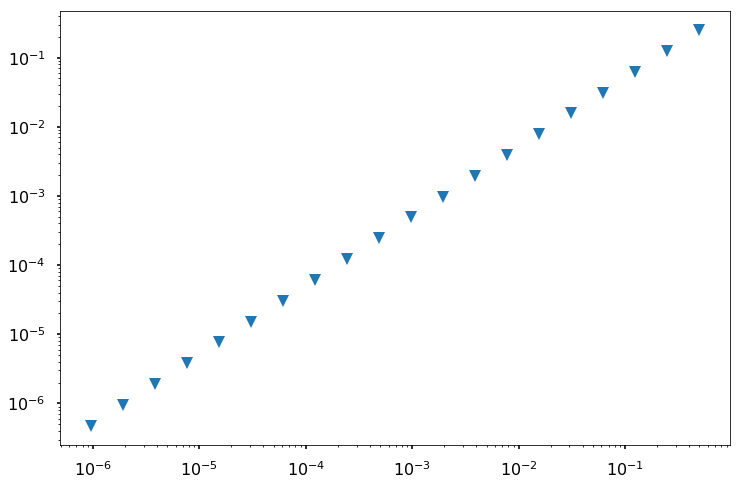
\includegraphics[width=13cm]{chapter20.02-Finite-Difference-Approximating-Derivatives_7_0}
%\caption{}
%\label{}
\end{center}
The slope of the line in log-log space is $1$; therefore, the error is proportional to $h^1$, which means that, as expected, the forward difference formula is $O(h)$.
\end{example}


%\begin{myexercise}\label{Comprehensionquiz2}
%%\begin{enumerate}[label=\arabic*.]
%%\item 
%%
%%\end{enumerate}
%\end{myexercise}

\section{Numerical Differentiation with Noise}
\videolesson
\begin{selfvideo}[2]
%LESSON 3: 
This video presents a discussion on numerical differentiation with noise. Follow the discussion and then solve the problems in the subsequent quiz.
\end{selfvideo}

As stated earlier, sometimes $f$ is given as a vector where $f$ is the corresponding function value for independent data values in another vector $x$, which is gridded. Sometimes data can be contaminated with {\bf noise}, meaning its value is off by a small amount from what it would be if it were computed from a pure mathematical function. This can often occur in engineering due to inaccuracies in measurement devices or the data itself can be slightly modified by perturbations outside the system of interest. For example, you may be trying to listen to your friend talk in a crowded room. The signal $f$ might be the intensity and tonal values in your friend’s speech. However, because the room is crowded, noise from other conversations are heard along with your friend’s speech, and he becomes difficult to understand.

To illustrate this point, we numerically compute the derivative of a simple cosine wave corrupted by a small sin wave. Consider the following two functions:
\[f(x)=\cos(x)\]
and
\[f_{\epsilon,\omega}(x)=\cos(x)+\epsilon\sin(\omega x)\]
where $0<\epsilon\ll1$ is a very small number and $\omega$ is a large number. When $\epsilon$ is small, it is clear that $f\simeq f_{\epsilon,\omega}$. To illustrate this point, we plot $f_{\epsilon,\omega}(x)$ for $\epsilon=0.01$ and $\omega=100$, and we can see it is very close to $f(x)$, as shown in the following figure.

\begin{boxB}
import numpy as np\\
import matplotlib.pyplot as plt\\
plt.style.use('seaborn-poster')\\
\%matplotlib inline
\end{boxB}

\begin{boxB}
x = np.arange(0, 2*np.pi, 0.01) \\
\# {\it compute function}\\
omega = 100\\
epsilon = 0.01\\
\\
y = np.cos(x) \\
y\_noise = y + epsilon*np.sin(omega*x)\\
\\
\# {\it Plot solution}\\
plt.figure(figsize = (12, 8))\\
plt.plot(x, y\_noise, 'r$^-$', \textbackslash \\
         \hspace*{1.5cm}label = 'cos(x) + noise')\\
plt.plot(x, y, 'b-', \textbackslash \\
         \hspace*{1.5cm}label = 'cos(x)')\\
\\
plt.xlabel('x')\\
plt.ylabel('y')\\
\\
plt.legend()\\
plt.show()\\
\end{boxB}

\begin{figure}[h]
\centering
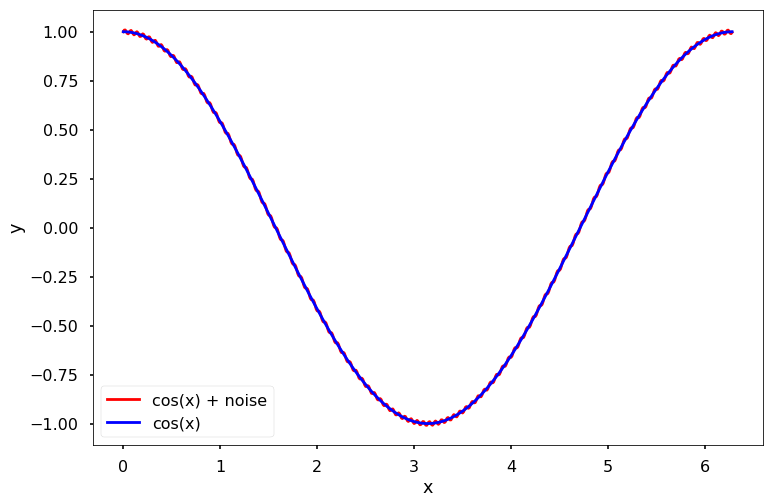
\includegraphics[width=13cm]{chapter20.04-Numerical-Differentiation-with-Noise_5_0}
\caption{}
\label{}
\end{figure}


The derivatives of our two test functions are
\[f'(x)=-\sin x\quad\mbox{ and }\quad f'_{\epsilon,\omega}(x)=-\sin x+\epsilon\omega\cos(\omega x).\]

Since $\epsilon\omega$ may not be small when $\omega$ is large, the contribution of the noise to the derivative may not be small. As a result, the derivative (analytic and numerical) may not be usable. For instance, the following figure shows $f'(x)$ and $f'_{\epsilon,\omega}(x)$ for $\epsilon=0.01$ and $\omega=100$.

\begin{boxB}
x = np.arange(0, 2*np.pi, 0.01) \\
\# compute function\\
y = -np.sin(x) \\
y\_noise = y + epsilon*omega*np.cos(omega*x)\\
\\
\# Plot solution\\
plt.figure(figsize = (12, 8))\\
plt.plot(x, y\_noise, 'r$^-$', \textbackslash \\
        \hspace*{1.5cm} label = 'Derivative cos(x) + noise')\\
plt.plot(x, y, 'b-', \textbackslash \\
        \hspace*{1.5cm} label = 'Derivative of cos(x)')\\
\\
plt.xlabel('x')\\
plt.ylabel('y')\\
\\
plt.legend()\\
plt.show()
\end{boxB}

\begin{figure}[h]
\centering
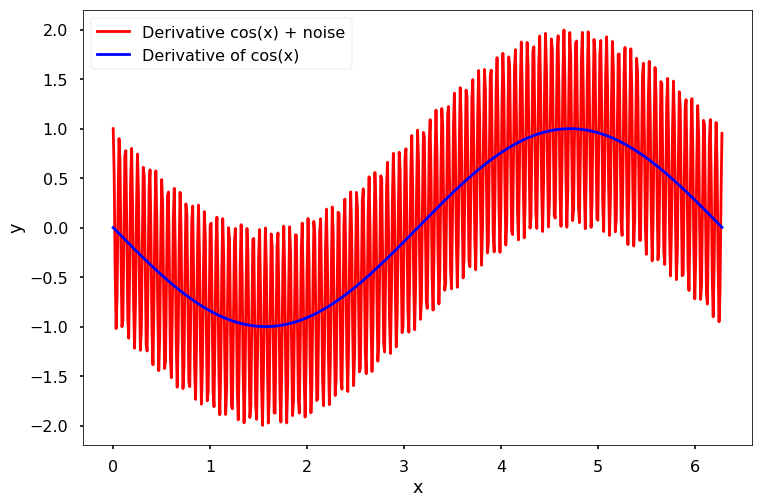
\includegraphics[width=12cm]{chapter20.04-Numerical-Differentiation-with-Noise_7_0}
\caption{}
\label{}
\end{figure}

%\begin{youtube}
%This video presents a discussion on numerical differentiation with noise. Follow the discussion and then solve the problems in the subsequent quiz.
%\end{youtube}


%\begin{myexercise}\label{Comprehensionquiz2}
%%\begin{enumerate}[label=\arabic*.]
%%\item 
%%
%%\end{enumerate}
%\end{myexercise}



\section{Riemann's Integral, Trapezoidal Rule and Simpson's Rule in Python}
\activities
Read stated reference on Riemann's integral, trapezoidal rule and Simpson's rule in python in the given web pages and then attempt the subsequent quiz.
\begin{activity}[\cg Reading]
\begin{enumerate}
\item Kong, Q., Siauw, T., Bayen, A., (2020). Python Programming and Numerical Methods. First Edition, Academic Press,  ISBN-13 ‏ : ‎ 978-0128195499 \\
\mylink{https://pythonnumericalmethods.studentorg.berkeley.edu/notebooks/chapter21.02-Riemanns-Integral.html}\\
\mylink{https://pythonnumericalmethods.studentorg.berkeley.edu/notebooks/chapter21.03-Trapezoid-Rule.html}
\mylink{https://pythonnumericalmethods.studentorg.berkeley.edu/notebooks/chapter21.04-Simpsons-Rule.html}
\end{enumerate}
\end{activity}
%\begin{myexercise}\label{Comprehensionquiz2}
%\begin{enumerate}[label=\arabic*.]
%\item 
%
%\end{enumerate}
%\end{myexercise}



%\begin{example}
%
%\end{example}
%
%\begin{mysolution}
%
%\end{mysolution}
%
%
%
%\begin{example}%\label{2ndorderpatderivative}
%
%\end{example}
%
%\begin{mysolution}
%
%\end{mysolution}



%\begin{myexercise}\label{Comprehensionquiz2}
%
%\end{myexercise}


\section{Computing Integrals in Python}
%\videolesson
%\begin{selfvideo}[2]
%%LESSON 3: 
%This video presents a discussion on computing integral in python. Follow the discussion and then solve the problems in the subsequent quiz.
%\end{selfvideo}
\begin{youtube}
This video presents a discussion on computing integral in python. Follow the discussion and then solve the problems in the subsequent quiz.
\end{youtube}
\mylink{https://www.youtube.com/watch?v=2I44Y9hfQ4Q}
%\begin{boxB}Question: \end{boxB}
%\begin{myexercise}\label{Comprehensionquiz2}
%%\begin{enumerate}[label=\arabic*.]
%%\item 
%%
%%\end{enumerate}
%\end{myexercise}


%\discussion


\begin{posttest}[\textcolor{red}{End of Module 9 Quiz}]
\item Consider the integral $\int_0^1x^2\,dx$. Using the trapezoidal rule write a python code for the definite integral and hence evaluate the integral
\item Find the work produced (𝑾) in a piston cylinder device using SciPy Module {\bf scipy.integrate}
\item Evaluate $\int_{-1}^1(𝑥^3 +2𝑥^2-𝑥+3)\,dx$ by writing a python code for both the indefinite and definite integrals.
\begin{mysolution}
\begin{enumerate}[label=\arabic*.]
\item ~\\
\begin{boxB}
import numpy as np\\
% import matplotlib.pyplot as plt\\
 a = 0; b = 1\\
 N = 10\\
\\
 x = np.linspace(a,b,N+1)\\
\\
 y = x**2;\\
\\
 y\_right = y[1:]\\
 y\_left = y[:-1]\\
\\
\# Trapezoid Rule\\
 dx = (b - a)/N\\
 A = (dx/2) * np.sum(y\_right + y\_left)\\
 print("A =", A)\\
%\\
%plt.plot(x,y)
% plt.xlim([0,1]); plt.ylim([0,1]);
\end{boxB}


\begin{boxB}
 import matplotlib.pyplot as plt\\
 import numpy as np\\
 xstart = 0\\
 xstop = 1.1\\
 increment = 0.1\\
\\
 x = np.arange(xstart, xstop, increment)\\
 y = x**2\\
\\
 plt.plot(x, y)\\
 plt.xlabel('x')\\
 plt.ylabel('y')\\
 plt.axis([0, 1, 0, 1])\\
 plt.fill\_between(x,y)\\
 plt.show()
\end{boxB}
\[f(x)=x^2\quad \int_0^1x^2\,dx=\frac13\approx0.3333\]


\begin{center}
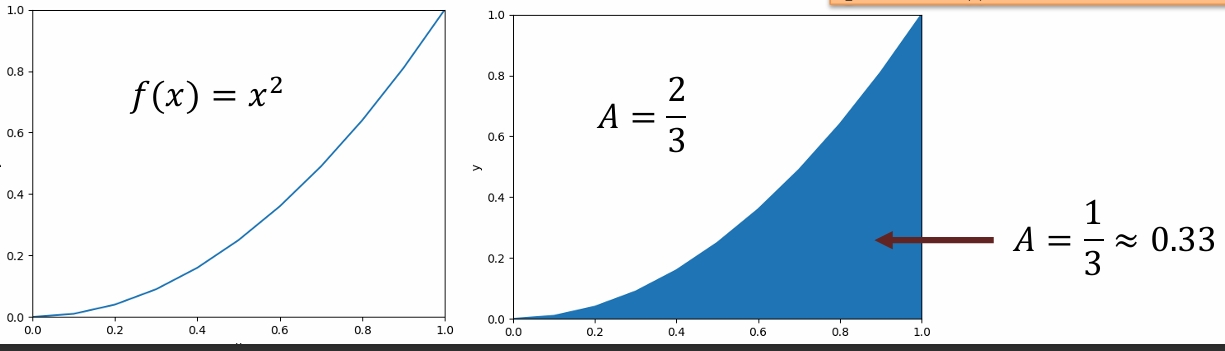
\includegraphics[width=15cm]{EndofMod9Q1sol}
\end{center}
Results from the Python code: $A = 0.3350000000000001$

\item ~\\
\begin{boxB}
from scipy import integrate\\
\\
 V1 = 1 \\
V2 = 5 \\
\\
n = 1\\
 R = 8.314\\
 T = 300\\
\\
 def work\_eq(V, n, R, T):\\
\hspace*{1cm} W = (n*R*T)/V  \\
\hspace*{1cm}return W\\
\\
 W, e = integrate.quad(work\_eq, V1, V2, args=(n, R, T,))\\
\\
 print("W =", W)
\end{boxB}

$W = 4014.2600411931353$

\item~\\
\begin{boxB}
import numpy.polynomial.polynomial as poly\\
\\
 p = [3, -1, 2, 1]\\
\\
 \# Find Indefinite integral\\
 I = poly.polyint(p)\\
 print("I =", I)\\

 \# Find Definite integral\\
 a = -1\\
 b = 1\\
\\
 A = poly.polyval(b, I) -poly.polyval(a, I)\\
 print("A =", A)
\end{boxB}

The Python solution: 
\[ I = [ 0.  3.  -0.5  0.66666667  0.25 ],\quad A = 7.333333333333333\]
\end{enumerate}
\end{mysolution}

\end{posttest}

%share your understanding of properties of functions and their applications to solving rates of change problems in physical phenomenon 


%\end{actsoln}

\takehome

\comy{You are now at the last part of this module. Your  task is to do a self-reflection on your learning experience.}



\references
\begin{refenumerate}
\item Kong, Q., Siauw, T., Bayen, A., (2020). Python Programming and Numerical Methods. First Edition, Academic Press,  ISBN-13 ‏ : ‎ 978-0128195499 \\
\mylink{https://pythonnumericalmethods.studentorg.berkeley.edu/notebooks/Index.html}
%chapter 1 pg 7-36 functions\\
%chapter 1 pg 51-83 limits and continuity\\
%chapter 1 pg 45-50 rates of change\\
%chapter 2 pg 108-120 the derivative\\
%\item Mendelson, E. (2022). Schaum's Outline of Calculus. McGraw-Hill Education.
%chapter 6 51-55 functions
%chapter 7 59-65 limits
%chapter 8 69-74 continuity
%chapter 9 77-81 derivative
%\item Calculus \mylink{https://math.libretexts.org/Bookshelves/Calculus}
%\item Chris McMullen, 2021, Essential Calculus Skills Practice Workbook with Full Solutions, Zishka Publishing, ISBN 978-1-941691-24-3
%\item R. Adams and C. Essex, 2021, Calculus: A complete Course, Addison Wesley, ISBN 13: 978-0135732588
%\item P. Abbott and H. Neill, 2018, Calculus: A Complete Introduction: The Easy Way to Learn Calculus (Teach Yourself), ISBN 13: 978-1473678446
\end{refenumerate}





%\wrapup
%To wrap-up, answer the following questions:
%
%\begin{enumerate}
%\item 
%%when do we say that a limit of a function exists?
%%\item how do we remove discontinuity in functions?
%%\item what is the relationship between the gradient of the tangent line and the derivative?
%\end{enumerate}
















%\newpage

%\facilitation


%
\begin{center}
    {\Large \textbf{FUNCTIONS OF SEVERAL VARIABLES}}\\[2mm]
(DEFINITION, DOMAIN, RANGE, GRAPHS AND LEVEL CURVES) \\[4mm]

\mycenterbox{5 minute review}%\\[4mm]
Recap the definition of a function of several variables, and the meaning of domain, range, graph and level curves of functions of several variables.
\end{center}
\mycenterbox{Warm-up.}%\\[4mm]
\problemAnswer{
Match the function with its graph (labeled I–VI).Give reasons for your choices
\begin{multicols}{3}
\begin{enumerate}[label=(\alph*)]
\item $f(x,y)=|x|+|y|$\\[4mm]
\item $f(x,y)=|xy|$
\item $f(x,y)=\frac{1}{1+x^2+y^2}$\\2mm]
\item $f(x,y)=(x^2-y^2)^2$
\item $f(x,y)=(x-y)^2$\\[4mm]
\item $f(x,y)=\sin(|x|+|y|)$
\end{enumerate}
\end{multicols}

\begin{center}
%\centering
\includegraphics[width=10cm]{MCTutorial1Q1.JPEG}
\end{center}
%\tcbox[tcbox raise base]{Warm-up}
 
%\begin{flushright}
%\begin{tikzpicture}
%    % A body
%
%
%    % Non-rectangle shapes must be drawn as polygone
%    \begin{scope}[shift={(3,0)}]
%        \draw  (0,0.5) -- (0,4) -- (.5,4) -- (.5,4.5) -- (1.,4.5) -- (4.,4.5) --(4.,4)-- (4.5,4) --(4.5,0.5) --(4.0,0.5)--(4.0,0.0)-- (.5,0) --(0.5,0.5) -- cycle;
%        % Draw symmetry lines
%        \draw [symmetry] (.5, 0.5) -- (.5,4.0);
%        \draw [symmetry] (4, 0.5) -- (4,4.0);
%        \draw [symmetry] (.5,4.0) -- (4,4.0);
%         \draw [symmetry] (.5, 0.5) -- (4, 0.5);
%        % Dimensions
%        \draw (4.5,0) -- ++(0.5,0) coordinate (D1) -- +(5pt,0);
%        \draw (4.5,4.5) -- ++(0.5,0) coordinate (D2) -- +(5pt,0);
%        \draw [dimen] (D1) -- (D2) node {6cm};
%       
%        
%        \draw (0.0,5) -- ++(0,0.5) coordinate (D1) -- +(0,+5pt);
%        \draw (0.5,5) -- ++(0,0.5) coordinate (D2) -- +(0,+5pt);
%        \draw [dimen,-] (D1) -- (D2) node [above=5pt] {$x$ cm};
%        \draw [dimen,<-] (D1) -- ++(-5pt,0);
%        \draw [dimen,<-] (D2) -- ++(+5pt,0);
%    \end{scope}
%\end{tikzpicture}
%\end{flushright}

}


\mycenterbox{Problems.}%

%\begin{center}
%\tcbox[tcbox raise base]{ Problems. Choose from the below}
%\end{center}
\problem{Exploring functions}%
\begin{enumerate}[(a)]
\item Are the following functions even, odd, or neither? What can you say
about their range?
\begin{multicols}{4}
 \begin{enumerate}[(i)]
\item $\displaystyle \frac{3x}{x^2+2}$
\item $\displaystyle \cos x+3$
\item $\displaystyle \frac{2x^3}{\cos x+3}$
\item $\displaystyle \frac{3x^4+2x^2}{\sin x+4}$
\end{enumerate}
\end{multicols}
\item Consider the functions $\sin^n x$ and $\cos^n x$, where $n$ is a positive integer.
Which are odd, which are even, and what are their periodicities?
\item What is the periodicity of $f(x) = 2 \cos x+\sin 2x$? Is it even/odd/neither?

\end{enumerate}

\problem{Cubic functions} 
Show that $x-1$ is a factor of the cubic function%
$$P(x)=x^3-2x^2-5x+6,$$
and  find the quadratic factor $Q(x)$ such that $P(x) = (x -1)Q(x)$. Factorise
$Q(x)$ and hence sketch $P(x).$

%\newpage
\problem{Sigmoid functions*.}%
For positive integers $n$, consider the family of functions
$$\displaystyle f_n= \frac{x^n}{2^n+x^n}.$$
\begin{enumerate}[(a)]
\item What are appropriate domains and ranges for $f_n(x)$? Do they depend on $n$?

\item Is $f_n(x)$ even, odd, or neither? Does this depend on $n$?

\item Show that for $x\geq 0$, $f_n(x)$ are strictly increasing functions and that
$0\leq f_n(x) < 1.$
\item What is the value of $f_n(2)$? Does it depend on $n$?

\item By considering the values of $f_n(1.9)$ and $f_n(2.1)$ for $n = 2, 4, 8, 16, 32$ and
$64$, show that the graph of $f_n(x)$ for $x\ge 0$ is an increasing sigmoid (that
is, $S$-shaped) function that approaches a step function as $n\rightarrow \infty$.
\end{enumerate}

\mycenterbox{Selected answers and hints}%

For the warm-up, $V(x)=4x(3-x)^2$. Writing $x=1+\epsilon$, we get
$$V = 4(1 +\epsilon)(3- (1+\epsilon))^2=4(4-\epsilon^2(3-\epsilon)).$$
If $-1<\epsilon<2$ then $\epsilon^2 (3-\epsilon)\ge 0$, with equality when $\epsilon=0$. Thus the maximum
value of $V$ occurs when $\epsilon= 0$, i.e. $x = 1\rm{cm}$.

\begin{enumerate}
\item 
\begin{enumerate}[(i)]
\item Odd. The range is the interval  $[-\frac{3}{4}\sqrt{2},\; \frac{3}{4}\sqrt{2}]$
\item Even. The range is the interval $[2, 4]$.
\item Odd. The range is all of $\mathbb R$.
\item Neither. (For example, writing $\displaystyle \frac{5}{\sin x+4}$ we have $\displaystyle f(1)= \frac{5}{\sin (1)+4} \equiv 1.032 (3\rm{dp})$ which is neither $f(1)$ nor $-f(1)$.)\\[4mm]
The range is the nonnegative reals $[0,\infty)$

\end{enumerate}
\end{enumerate}










